\chapter{Bài toán đếm Polya}

\section{Bổ đề Burnside}

\subsection*{Lớp tương đương}

Xét nhóm $G$ và tập hợp $M$. Khi đó hai phần tử $m$ và $n$ thuộc $M$ được gọi là \textbf{quan hệ với nhau} nếu tồn tại $g \in G$ mà $m = g n$.

\begin{remark}
    Quan hệ giữa các phần tử như trên là quan hệ tương đương.    
\end{remark}

\begin{proof}
    Để chứng minh một quan hệ là tương đương, ta cần chứng minh tính phản xạ, đối xứng và bắc cầu.

    Đối với tính phản xạ, mọi vector đều có quan hệ với chính nó qua phần tử đơn vị $e \in G$.

    Đối với tính đối xứng, nếu $m$ có quan hệ với $n$ thì tồn tại $g \in G$ sao cho $m = gn$. Theo tính chất nhóm thì tồn tại phần tử $g^{-1}$ là nghịch đảo của $g$ trong $G$. Do đó $g^{-1} m = n$. Nói cách khác $n$ cũng có quan hệ với $m$. Như vậy ta có tính đối xứng.

    Đối với tính bắc cầu, nếu $m$ có quan hệ với $n$ thì tồn tại $g_1 \in G$ sao cho $m = g_1 n$. Tiếp theo, nếu $n$ có quan hệ với $p$ thì tồn tại $g_2 \in G$ sao cho $n = g_2 p$. Suy ra $m = g_1 n = g_1 (g_2 p) = (g_1 g_2) p$. Do $g_1, g_2 \in G$ nên $g_1 g_2 \in G$. Như vậy $m$ cũng có quan hệ với $p$ nên quan hệ có tính bắc cầu.

    Vậy quan hệ được định nghĩa như trên là quan hệ tương đương.
\end{proof}

\subsection*{Tác động nhóm lên vector}

Xét nhóm $G$ và không gian vector $\FF_2^n$, $n \in \NN$. Khi đó hai vector $\bm{x}$ và $\bm{y}$ thuộc $\FF_2^n$ được gọi là \textbf{quan hệ với nhau} nếu tồn tại $g \in G$ mà $\bm{x} = g \bm{y}$.

Ví dụ, xét nhóm hoán vị $\mathcal{S}_3$. Giả sử các vector trong $\FF_2^3$ có dạng \[ \bm{x} = (x_1, x_2, x_3) \in \FF_2^3. \] 

Khi đó vector $(1, 0, 0)$ có quan hệ với $(0, 0, 1)$ với hoán vị $(1, 3)(2)$. Cụ thể là $(x_1, x_2, x_3) \xrightarrow{(1, 3)(2)} (x_3, x_2, x_1)$.

Tương tự, vector $(1, 0, 0)$ cũng có quan hệ với $(0, 1, 0)$ với hoán vị $(1, 2)(3)$. Thêm nữa, vector $(1, 0, 0)$ có quan hệ với chính nó qua hoán vị đồng nhất $(1)(2)(3)$.

Trong môn toán rời rạc ta đã biết, nếu một tập có quan hệ tương đương thì ta có thể phân các phần tử của tập đó vào các lớp tương đương rời nhau. Nghĩa là nếu hai phần tử có quan hệ với nhau thì vào cùng một lớp tương đương. Từ phần trên ta đã biết rằng dưới tác động của nhóm, các phần tử trong tập hợp bất kì sẽ phân bổ thành các lớp tương đương.

Câu hỏi đặt ra là, có bao nhiêu lớp tương đương như vậy?

Để giải quyết vấn đề này ta sử dụng bổ đề Burnside.

Nhóm $\mathcal{S}_3$ có các hoán vị \[ \mathcal{S}_3 = \{ (1)(2)(3), (1, 2)(3), (1, 3)(2), (2, 3)(1), (1, 3, 2), (1, 2, 3) \} \]

Lần lượt xét từng hoán vị. Đầu tiên, với $(1)(2)(3)$ thì các phần tử trong vector đứng yên. Do đó dưới tác động của hoán vị này, $x_1$ biến thành $x_1$, $x_2$ biến thành $x_2$ và $x_3$ biến thành $x_3$. Số cách chọn cho mỗi $x_i$ là 2 nên theo quy tắc nhân ta có $2^3 = 8$ cách.

Tiếp theo, với hoán vị $(1, 2)(3)$ thì $x_1 \to x_2$, $x_2 \to x_1$ và $x_3 \to x_3$. Do đó $x_1$ và $x_2$ có cùng giá trị nên có 2 cách chọn, $x_3$ cũng có 2 cách chọn nên tổng số cách là $2 \cdot 2 = 4$. Hoán vị $(1, 3)(2)$ và $(2, 3)(1)$ tương tự.

Với hoán vị $(1, 2, 3)$ thì $x_1 \to x_2$, $x_2 \to x_3$ và $x_3 \to x_1$ nên $x_1 = x_2 = x_3$, có 2 cách chọn trong trường hợp này. Hoán vị $(1, 3, 2)$ tương tự.

Như vậy, theo bổ đề Burnside, số lớp tương đương các vector trong $\FF_2^3$ là \[ t(\mathcal{S}_3) = \frac{1}{6} (1 \cdot 2^3 + 3 \cdot 2^2 + 2 \cdot 2) = 4 \]

Thật vậy, ta có thể chia các vector thành 4 lớp tương đương là $\{ 000 \}$, $\{ 001, 010, 011 \}$, $\{ 011, 101, 110 \}$, $\{ 111 \}$.

Ngoài nhóm $\mathcal{S}_3$ ra còn các nhóm khác cũng tác động lên các vector. Một số nhóm hay được sử dụng là:

\begin{enumerate}
    \item Nhóm general linear: gồm các ma trận khả nghịch $n \times n$ trên $\FF_2$. Tác động nhóm lúc này là phép nhân ma trận $\bm{A} \in GL(n, 2)$ với vector $\bm{x} \in \FF_2^n$, hay $\bm{A} \cdot \bm{x}$.
    \item Nhóm general affine: gồm các ma trận khả nghịch $n \times n$ trên $\FF_2$ và vector bất kì trong $\FF_2^n$. Tác động nhóm lúc này là biến đổi affine $\bm{A} \cdot \bm{x} + \bm{b}$ với $\bm{A} \in GL(n, 2)$ và $\bm{b} \in \FF_2^n$.
\end{enumerate}

%Cần nhắc lại một chút, số lượng phần tử của nhóm $GL(n, 2)$ là \[ (2^n - 1) \cdot (2^n - 2) \cdots (2^n - 2^{n-1}) \]

%Khi $n = 3$ thì $\lvert GL(3, 2) \rvert = (2^3 - 1) \cdot (2^3 - 2) \cdot (2^3 - 4) = 168$ ma trận.

\subsection*{Tác động nhóm lên hàm boolean}

Ta tiếp tục xét nhóm $G$ và không gian vector $\FF_2^n$, $n \in \NN$. Khi đó hai hàm boolean $n$ biến $f(x_1, \ldots, x_n)$ và $g(x_1, \ldots, x_n)$ được gọi là \textbf{quan hệ với nhau} nếu tồn tại $g \in G$ mà $g(\bm{x}) = f(g \bm{x})$ với mọi $\bm{x} \in \FF_2^n$.

Ta cũng xét hoán vị $\mathcal{S}_3$. Ta cũng lần lượt xét các phần tử của nhóm.

Đặt $f_0, f_1, \ldots, f_7$ lần lượt là các giá trị hàm $f$ với các vector $\bm{x} \in \FF_2^3$.

Đầu tiên, với $(1)(2)(3)$, ta có bảng chuyển vector như hình \ref{burnside:first}.

\begin{figure}[ht]
    \centering
    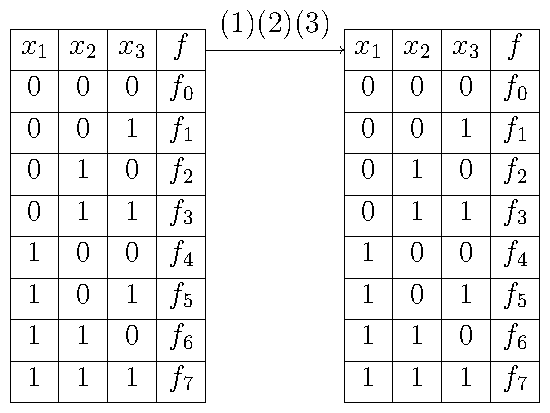
\includegraphics[page=1]{figures/burnside.pdf}
    \caption{Hoán vị $(1)(2)(3)$}
    \label{burnside:first}
\end{figure}

Ta thấy rằng $f_0 \to f_0$, $f_1 \to f_1$, ..., $f_7 \to f_7$ nên có 8 chu trình. Vậy số lượng cách chọn là $2^8$.

Tiếp theo, xét các hoán vị dạng $(1)(2, 3)$, ta có bảng chuyển vector như hình \ref{burnside:second}.

\begin{figure}[ht]
    \centering
    \includegraphics[page=2]{figures/burnside.pdf}
    \caption{Hoán vị $(1)(2, 3)$}
    \label{burnside:second}
\end{figure}

Ta thấy rằng $f_0 \to f_0$, $f_1 \to f_2 \to f_1$, $f_3 \to f_3$, $f_4 \to f_4$, $f_5 \to f_6 \to f_5$, $f_7 \to f_7$. Ở đây có 6 chu trình nên số cách chọn là $2^6$.

Tiếp theo ta xét các hoán vị dạng $(1, 2, 3)$ (hình \ref{burnside:third}).

\begin{figure}[ht]
    \centering
    \includegraphics[page=3]{figures/burnside.pdf}
    \caption{Hoán vị $(1, 2, 3)$}
    \label{burnside:third}
\end{figure}

Ta thấy rằng $f_0 \to f_0$, $f_1 \to f_2 \to f_4 \to f_1$, $f_3 \to f_6 \to f_5 \to f_3$, $f_7 \to f_7$ nên ở đây có 4 chu trình. Số cách chọn là $2^4$.

Như vậy theo bổ đề Burnside, số lớp hàm bool tương đương dưới tác động của nhóm $\mathcal{S}_3$ là \[ t (\mathcal{S}_3) = \dfrac{1}{6}(2^8 + 3 \cdot 2^6 + 2 \cdot 2^4) = 80. \]
